\chapter{Solução Proposta}
\label{cap:solucao-proposta}

Este capítulo apresenta a solução proposta para apoiar os discentes na organização do barema de atividades complementares conforme discutido na Seção \ref{sec:desafios}. A solução consiste em um sistema web que centraliza o preenchimento dos dados do aluno, a anexação dos certificados, a pré-validação das informações e a geração de um documento final em PDF.

\section{Visão Geral da Solução}

O sistema foi concebido para atuar antes da submissão oficial do barema (descrita em \ref{sec:definicao}), funcionando como uma camada de apoio à organização e conferência inicial dos documentos. O discente informa seus dados, seleciona o tipo de barema, preenche as cargas horárias solicitadas e anexa os certificados correspondentes a cada atividade. A partir dessas informações, a aplicação verifica inconsistências básicas, organiza os arquivos e gera um PDF consolidado.

Importante observar que esta proposta não substitui a análise institucional realizada pelo colegiado. Seu objetivo é reduzir erros comuns no envio, como carga horária incompatível, certificados repetidos, ausência de informações mínimas e desorganização dos anexos (descritos na Seção \ref{sec:desafios}). Assim, o sistema contribui para que o discente entregue um material mais consistente e para que a etapa posterior de conferência seja menos sujeita a retrabalho.

\section{Interface do Sistema}

A interface do sistema foi organizada para conduzir o discente pelo fluxo de preenchimento do barema de forma progressiva. Inicialmente, o usuário acessa uma tela de apresentação com a identificação da finalidade da ferramenta e um formulário para inserção dos dados básicos, como nome, matrícula, e-mail e data de verificação. Essa etapa é importante porque a matrícula permite ao sistema identificar automaticamente o regulamento aplicável ao discente.

\begin{figure}[H]
    \centering
    \caption{Tela inicial do sistema Barema.}
    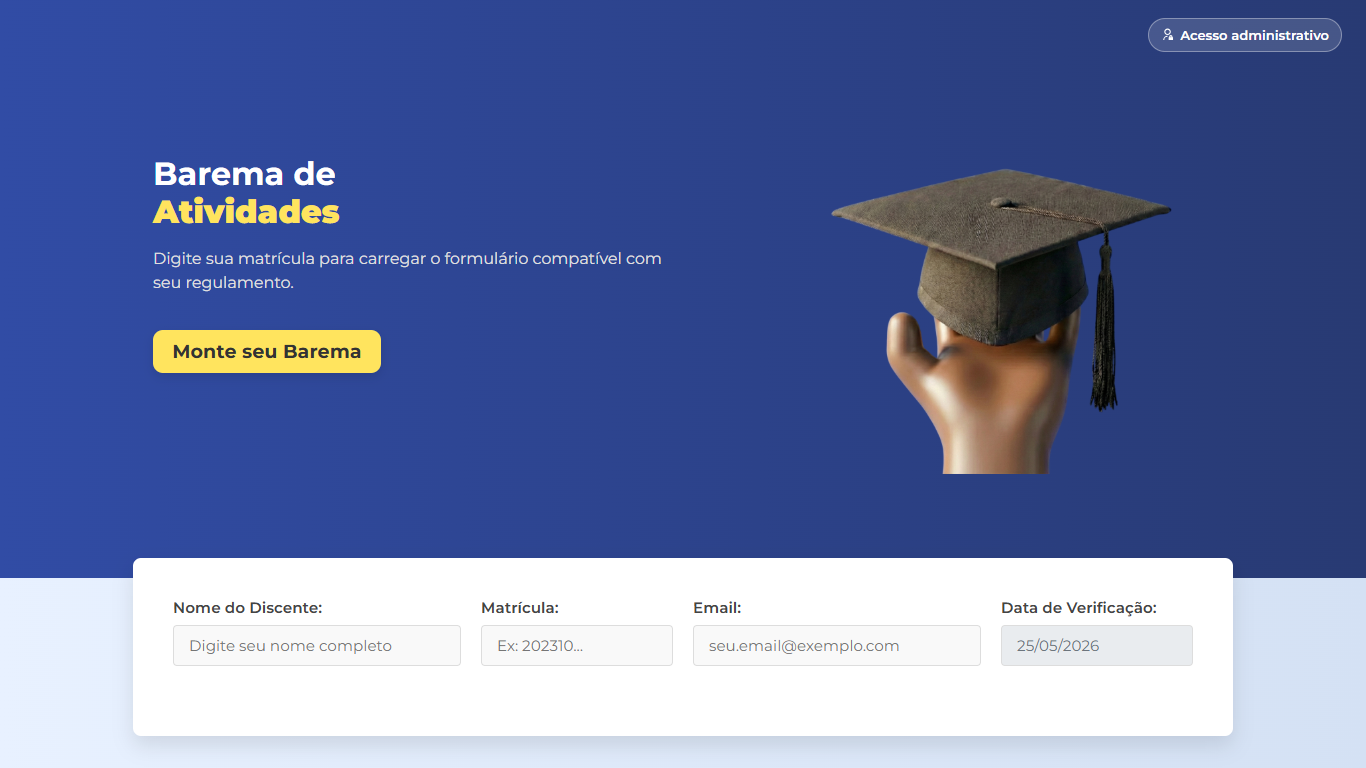
\includegraphics[width=0.9\textwidth]{figuras/telas/01_tela_inicial_barema.png}
    \legend{Fonte: elaboração própria.}
    \label{fig:tela-inicial-barema}
\end{figure}

Após o preenchimento da matrícula, o sistema carrega dinamicamente a tabela de atividades correspondente ao barema do aluno. Nessa tela, o discente informa a carga horária cumprida em cada atividade e anexa os comprovantes em formato PDF. A organização em tabela aproxima a interface da estrutura do documento final, facilitando a conferência das informações antes da geração do arquivo consolidado.

\begin{figure}[H]
    \centering
    \caption{Formulário do barema com atividades carregadas.}
    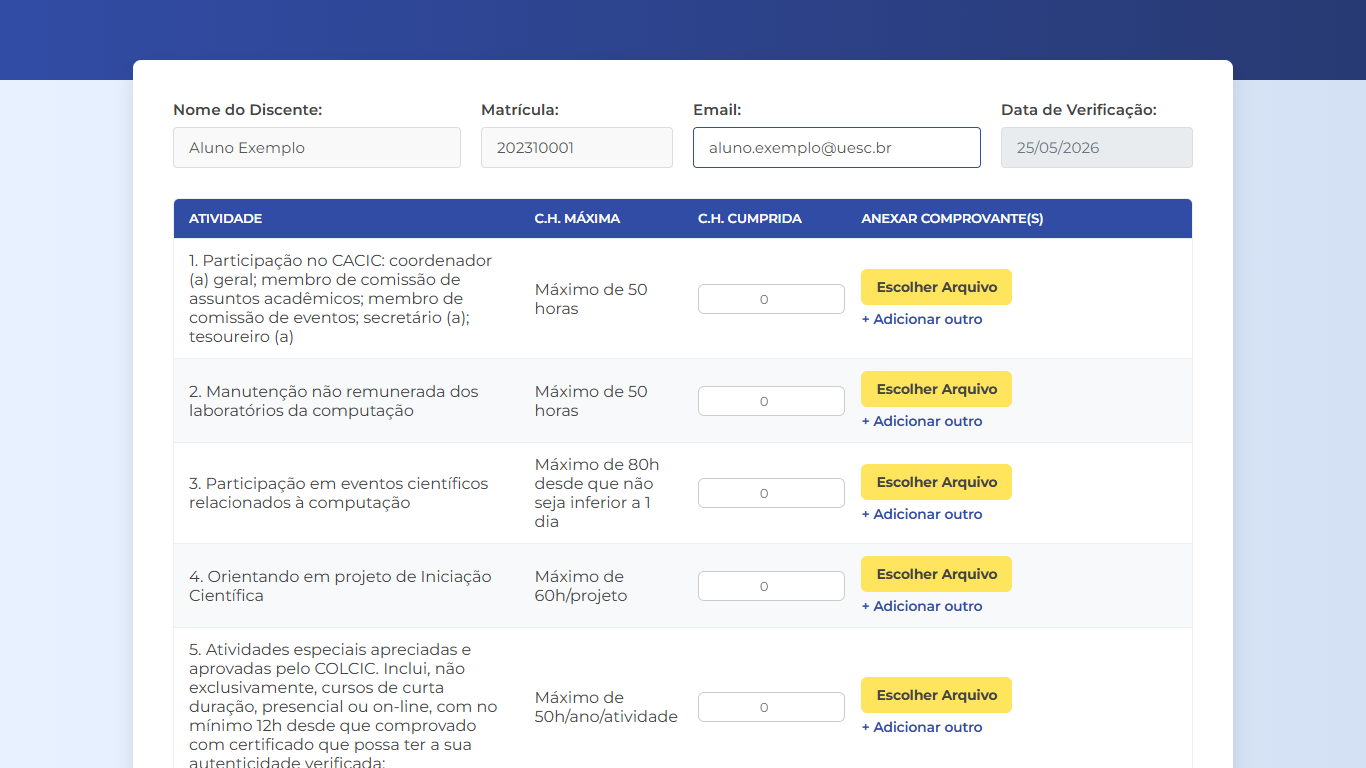
\includegraphics[width=0.9\textwidth]{figuras/telas/02_formulario_com_tabela.png}
    
    \legend{Fonte: elaboração própria.}
    \label{fig:formulario-barema}
\end{figure}

Além da interface voltada ao discente, o sistema possui uma tela de autenticação administrativa. Esse acesso é destinado à coordenação ou aos responsáveis pelo acompanhamento das solicitações, separando o fluxo público de preenchimento do barema das funcionalidades restritas de gestão.

\begin{figure}[H]
    \centering
    \caption{Tela de login administrativo.}
    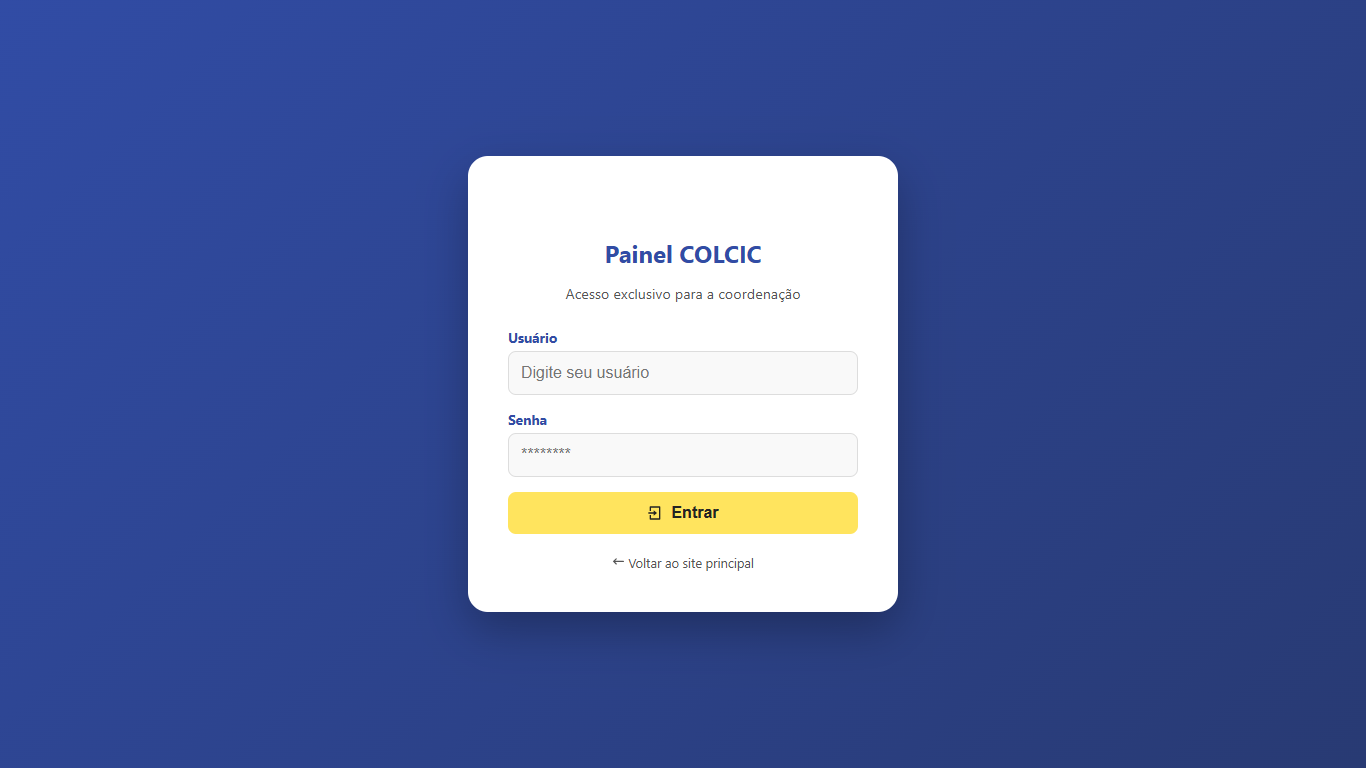
\includegraphics[width=0.9\textwidth]{figuras/telas/03_login_administrativo.png}
    
    \legend{Fonte: elaboração própria.}
    \label{fig:login-administrativo}
\end{figure}

Após a autenticação, o coordenador acessa o painel de solicitações de análise. Essa interface concentra os registros enviados pelos discentes, permite filtrar solicitações por status, abrir o documento unificado submetido e registrar o parecer que será encaminhado ao aluno.

\begin{figure}[H]
    \centering
    \caption{Painel do coordenador para análise das solicitações.}
    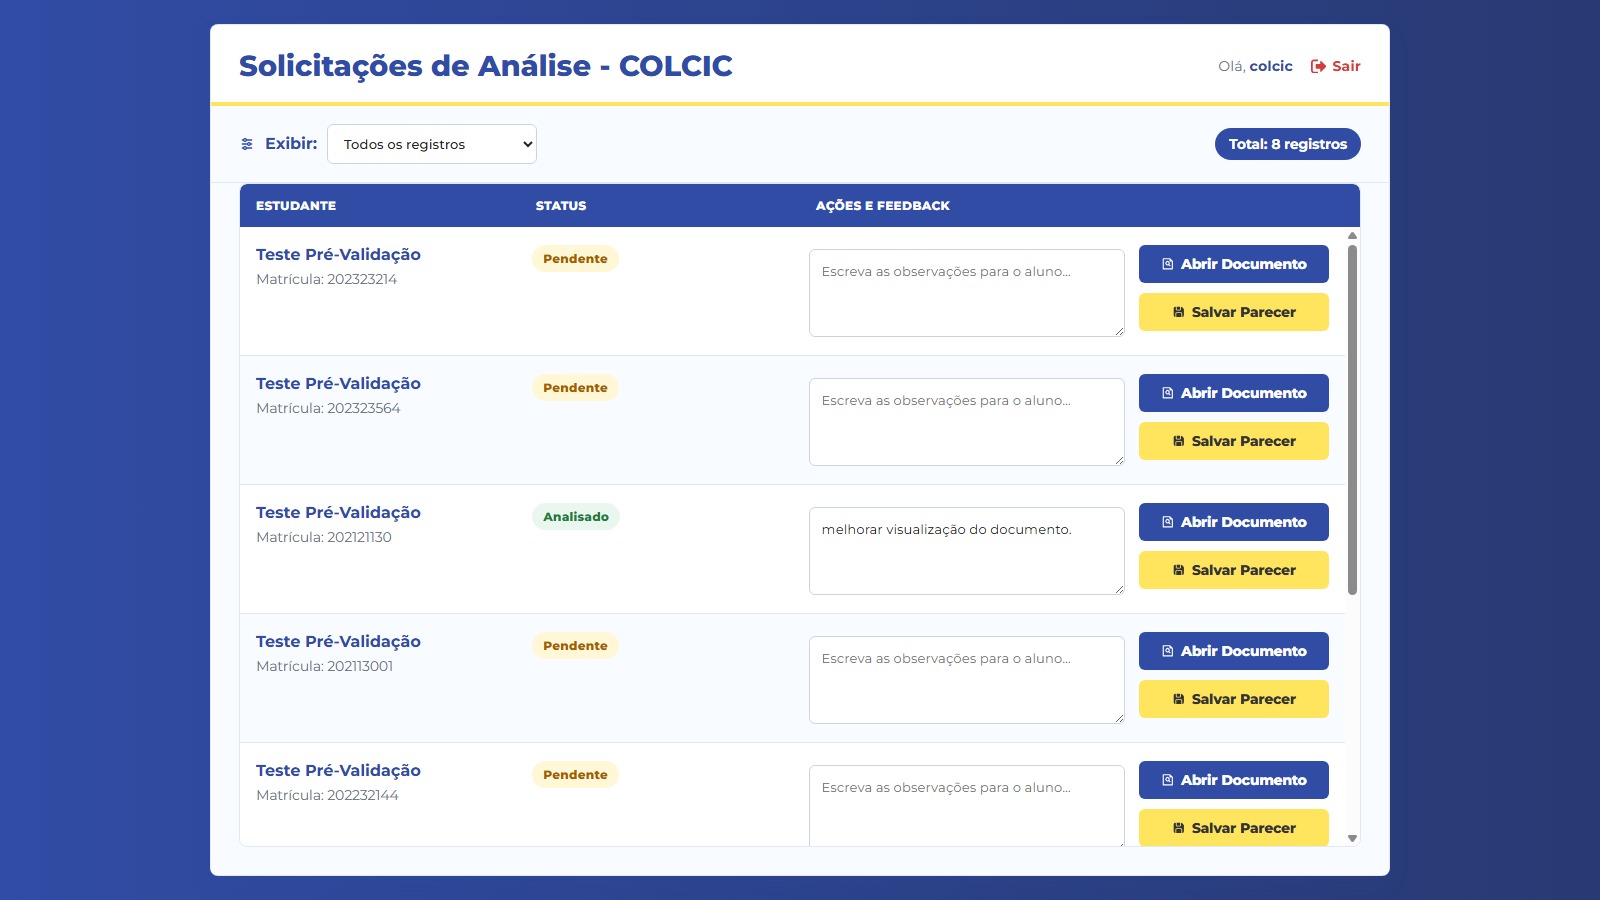
\includegraphics[width=0.9\textwidth]{figuras/telas/04_painel_coordenador.png}
    
    \legend{Fonte: elaboração própria.}
    \label{fig:painel-coordenador}
\end{figure}

\section{Arquitetura e Fluxo de Funcionamento}

A aplicação foi estruturada em camadas para separar responsabilidades. A interface web concentra a interação com o usuário, incluindo preenchimento do formulário, anexação e remoção de arquivos e \textit{feedbacks} visuais. As rotas da aplicação recebem os dados enviados pelo navegador e acionam os serviços responsáveis pelo processamento. A camada de serviços realiza a extração de informações dos certificados, aplica regras de pré-validação, organiza os dados do barema e encaminha a geração do PDF final.

No \textit{backend}, a implementação utiliza Python\texttrademark{} e Flask\texttrademark{}, com serviços especializados para processamento de certificados, validação e geração de documentos. A leitura dos arquivos PDF é feita de forma transiente, evitando que os certificados individuais precisem ser mantidos permanentemente no servidor durante o fluxo de geração. O sistema também conta com uma área administrativa para acompanhamento das solicitações registradas, quando essa etapa for utilizada no fluxo de operação.

Essa organização em camadas facilita a evolução do sistema, pois permite alterar a interface, as regras de validação ou o mecanismo de geração de documentos sem misturar responsabilidades. Também favorece a realização de testes unitários sobre regras específicas, como extração de carga horária, comparação de horas solicitadas e identificação de duplicidade.

\section{Pré-validação e Geração do Barema}

Um dos componentes centrais da solução é a pré-validação dos certificados. A validação básica verifica informações objetivas, como presença do nome do aluno, carga horária extraída, compatibilidade entre horas solicitadas e comprovadas e duplicidade de certificados. Além disso, o sistema foi preparado para utilizar uma camada opcional de inteligência artificial, configurável por provedor externo, para apoiar análises textuais mais flexíveis sobre o conteúdo dos certificados.

Quando a inteligência artificial está habilitada e disponível, ela pode complementar a análise da relação entre o certificado e a atividade declarada. Caso o serviço externo esteja indisponível ou mal configurado, o sistema retorna automaticamente à validação básica, preservando o funcionamento do fluxo. Essa decisão evita que a ferramenta dependa exclusivamente de recursos externos para orientar o discente.

Após a pré-validação, a solução consolida os dados preenchidos e os comprovantes anexados em um único documento PDF. O arquivo gerado organiza as atividades e seus certificados de forma padronizada, permitindo que o aluno tenha uma versão final mais clara, completa e adequada para encaminhamento à análise oficial.
